\section{Análisis de factibilidad del ciclo oficial de cinco descargas diarias con chaqueta de 14~m\textsuperscript{2}}
\label{sec:ciclo_12m3h}

El presente análisis evalúa la factibilidad térmica del ciclo operativo oficial del tanque de almacenamiento de glucosa Tag 53A-90A-0056. El ciclo consiste en cinco descargas diarias de 24~ton de glucosa cada una, bombeadas durante 2,0~h a un flujo másico de 12~ton/h, con un período de ciclo de 4,80~h entre inicios de descarga. Se considera una chaqueta de media caña con área de transferencia de 14~m\textsuperscript{2}, agua de calentamiento a 75~\textdegree C, velocidad del agua de 2,5~m/s y configuración de doble entrada. Entre descargas no se programan tiempos muertos; los 2,80~h restantes se destinan exclusivamente a calentamiento.

\subsection{Supuestos de diseño del ciclo}

El modelo adopta las bases de diseño congeladas del proyecto W2605. La Tabla~\ref{tab:parametros_ciclo_oficial} resume los datos de entrada.

\begin{table}[H]
\centering
\caption{Parámetros del ciclo oficial de descargas evaluado con chaqueta de 14~m\textsuperscript{2}.}
\label{tab:parametros_ciclo_oficial}
\begin{tabular}{@{}lcc@{}}
\toprule
\textbf{Parámetro} & \textbf{Valor} & \textbf{Unidad} \\
\midrule
Área de transferencia de la chaqueta & 14 & m\textsuperscript{2} \\
Temperatura del agua de calentamiento & 75 & \textdegree C \\
Velocidad del agua en la media caña & 2,5 & m/s \\
Flujo másico de descarga & 12 & ton/h \\
Flujo volumétrico de descarga a 55~\textdegree C & 8,54 & m\textsuperscript{3}/h \\
Masa de glucosa por descarga & 24 & ton \\
Duración de cada descarga & 2,0 & h \\
Período de ciclo entre inicios de descarga & 4,80 & h \\
Tiempo de calentamiento entre descargas & 2,80 & h \\
Temperatura de la glucosa de alimentación & 55 & \textdegree C \\
Nivel inicial del tanque & 80 & \% \\
Temperatura inicial del tanque & 60 & \textdegree C \\
Temperatura mínima de despacho & 57 & \textdegree C \\
\bottomrule
\end{tabular}
\end{table}

El volumen de glucosa que corresponde a 24~ton a 55~\textdegree C se calcula mediante la densidad del jarabe Globe 1130:

\begin{equation}
V_d = \frac{m_d}{\rho_g(55\textdegree C)} = \frac{24~000~\text{kg}}{1405,7~\text{kg/m}^3} = 17,07~\text{m}^3
\label{eq:volumen_descarga_oficial}
\end{equation}

Por tanto, el flujo volumétrico de descarga resulta:

\begin{equation}
\dot{V}_d = \frac{\dot{m}_d}{\rho_g(55\textdegree C)} = \frac{12~000~\text{kg/h}}{1405,7~\text{kg/m}^3} = 8,54~\text{m}^3/\text{h}
\label{eq:flujo_volumetrico_oficial}
\end{equation}

La duración de cada descarga, con el flujo másico oficial de 12~ton/h, es:

\begin{equation}
t_d = \frac{m_d}{\dot{m}_d} = \frac{24~000~\text{kg}}{12~000~\text{kg/h}} = 2,00~\text{h}
\label{eq:duracion_descarga_oficial}
\end{equation}

Con cinco descargas distribuidas en 24~h, el período de ciclo disponible es 4,80~h, dejando un tiempo de calentamiento entre descargas de 2,80~h.

\subsection{Modelo matemático}

Durante la descarga, el tanque recibe glucosa a 55~\textdegree C al mismo flujo másico con el que se retira glucosa hacia el carrotanque, por lo que la masa de líquido en el tanque permanece aproximadamente constante. El balance de energía transitorio se expresa como:

\begin{equation}
m_g \, C_{p,g}(T_g) \, \frac{dT_g}{dt} = U(T_g) \, A \, (T_a - T_g) + \dot{m}_{in} \, C_{p,g}(55\textdegree C) \, (55 - T_g) - Q_{perd}(T_g)
\label{eq:balance_descarga_oficial}
\end{equation}

Entre descargas no existe flujo de entrada ni salida, por lo que el balance se reduce a:

\begin{equation}
m_g \, C_{p,g}(T_g) \, \frac{dT_g}{dt} = U(T_g) \, A \, (T_a - T_g) - Q_{perd}(T_g)
\label{eq:balance_calentamiento_oficial}
\end{equation}

donde $m_g$ es la masa de glucosa en el tanque, $U(T_g)$ el coeficiente global dependiente de la temperatura, $A = 14~\text{m}^2$, $T_a = 75~\textdegree C$, $\dot{m}_{in}$ el flujo másico de alimentación y $Q_{perd}(T_g)$ las pérdidas térmicas al ambiente calculadas con el área real expuesta y el aislamiento de lana mineral de 50,8~mm.

\subsection{Resultados de la simulación}

La integración numérica de las ecuaciones~\eqref{eq:balance_descarga_oficial} y \eqref{eq:balance_calentamiento_oficial} se realizó mediante el método RK45 con paso adaptativo, actualizando las propiedades termofísicas de la glucosa y el coeficiente $U$ en cada instante. La Tabla~\ref{tab:resultados_ciclo_oficial} presenta la temperatura del tanque al inicio y al final de cada descarga.

\begin{table}[H]
\centering
\caption{Evolución de la temperatura del tanque durante las cinco descargas diarias del ciclo oficial (flujo de 12~ton/h, área de 14~m\textsuperscript{2}).}
\label{tab:resultados_ciclo_oficial}
\begin{tabular}{@{}cccccc@{}}
\toprule
\textbf{Descarga} & \textbf{$t_{inicio}$ [h]} & \textbf{$t_{fin}$ [h]} & \textbf{$T_{inicial}$ [\textdegree C]} & \textbf{$T_{final}$ [\textdegree C]} & \textbf{Cumple $T \geq 57$~\textdegree C} \\
\midrule
1 & 0,00 & 2,00 & 60,00 & 59,59 & Sí \\
2 & 4,80 & 6,80 & 59,66 & 59,29 & Sí \\
3 & 9,60 & 11,60 & 59,36 & 59,02 & Sí \\
4 & 14,40 & 16,40 & 59,09 & 58,77 & Sí \\
5 & 19,20 & 21,20 & 58,86 & 58,56 & Sí \\
\bottomrule
\end{tabular}
\end{table}

La temperatura mínima alcanzada durante todo el ciclo es 58,56~\textdegree C, registrada al finalizar la quinta descarga. La temperatura final del tanque al cabo de las 24~h es 58,64~\textdegree C. La Figura~\ref{fig:ciclo_oficial_T_vs_t} ilustra el perfil transitorio de temperatura y el nivel del tanque durante el día de operación.

\begin{figure}[H]
\centering
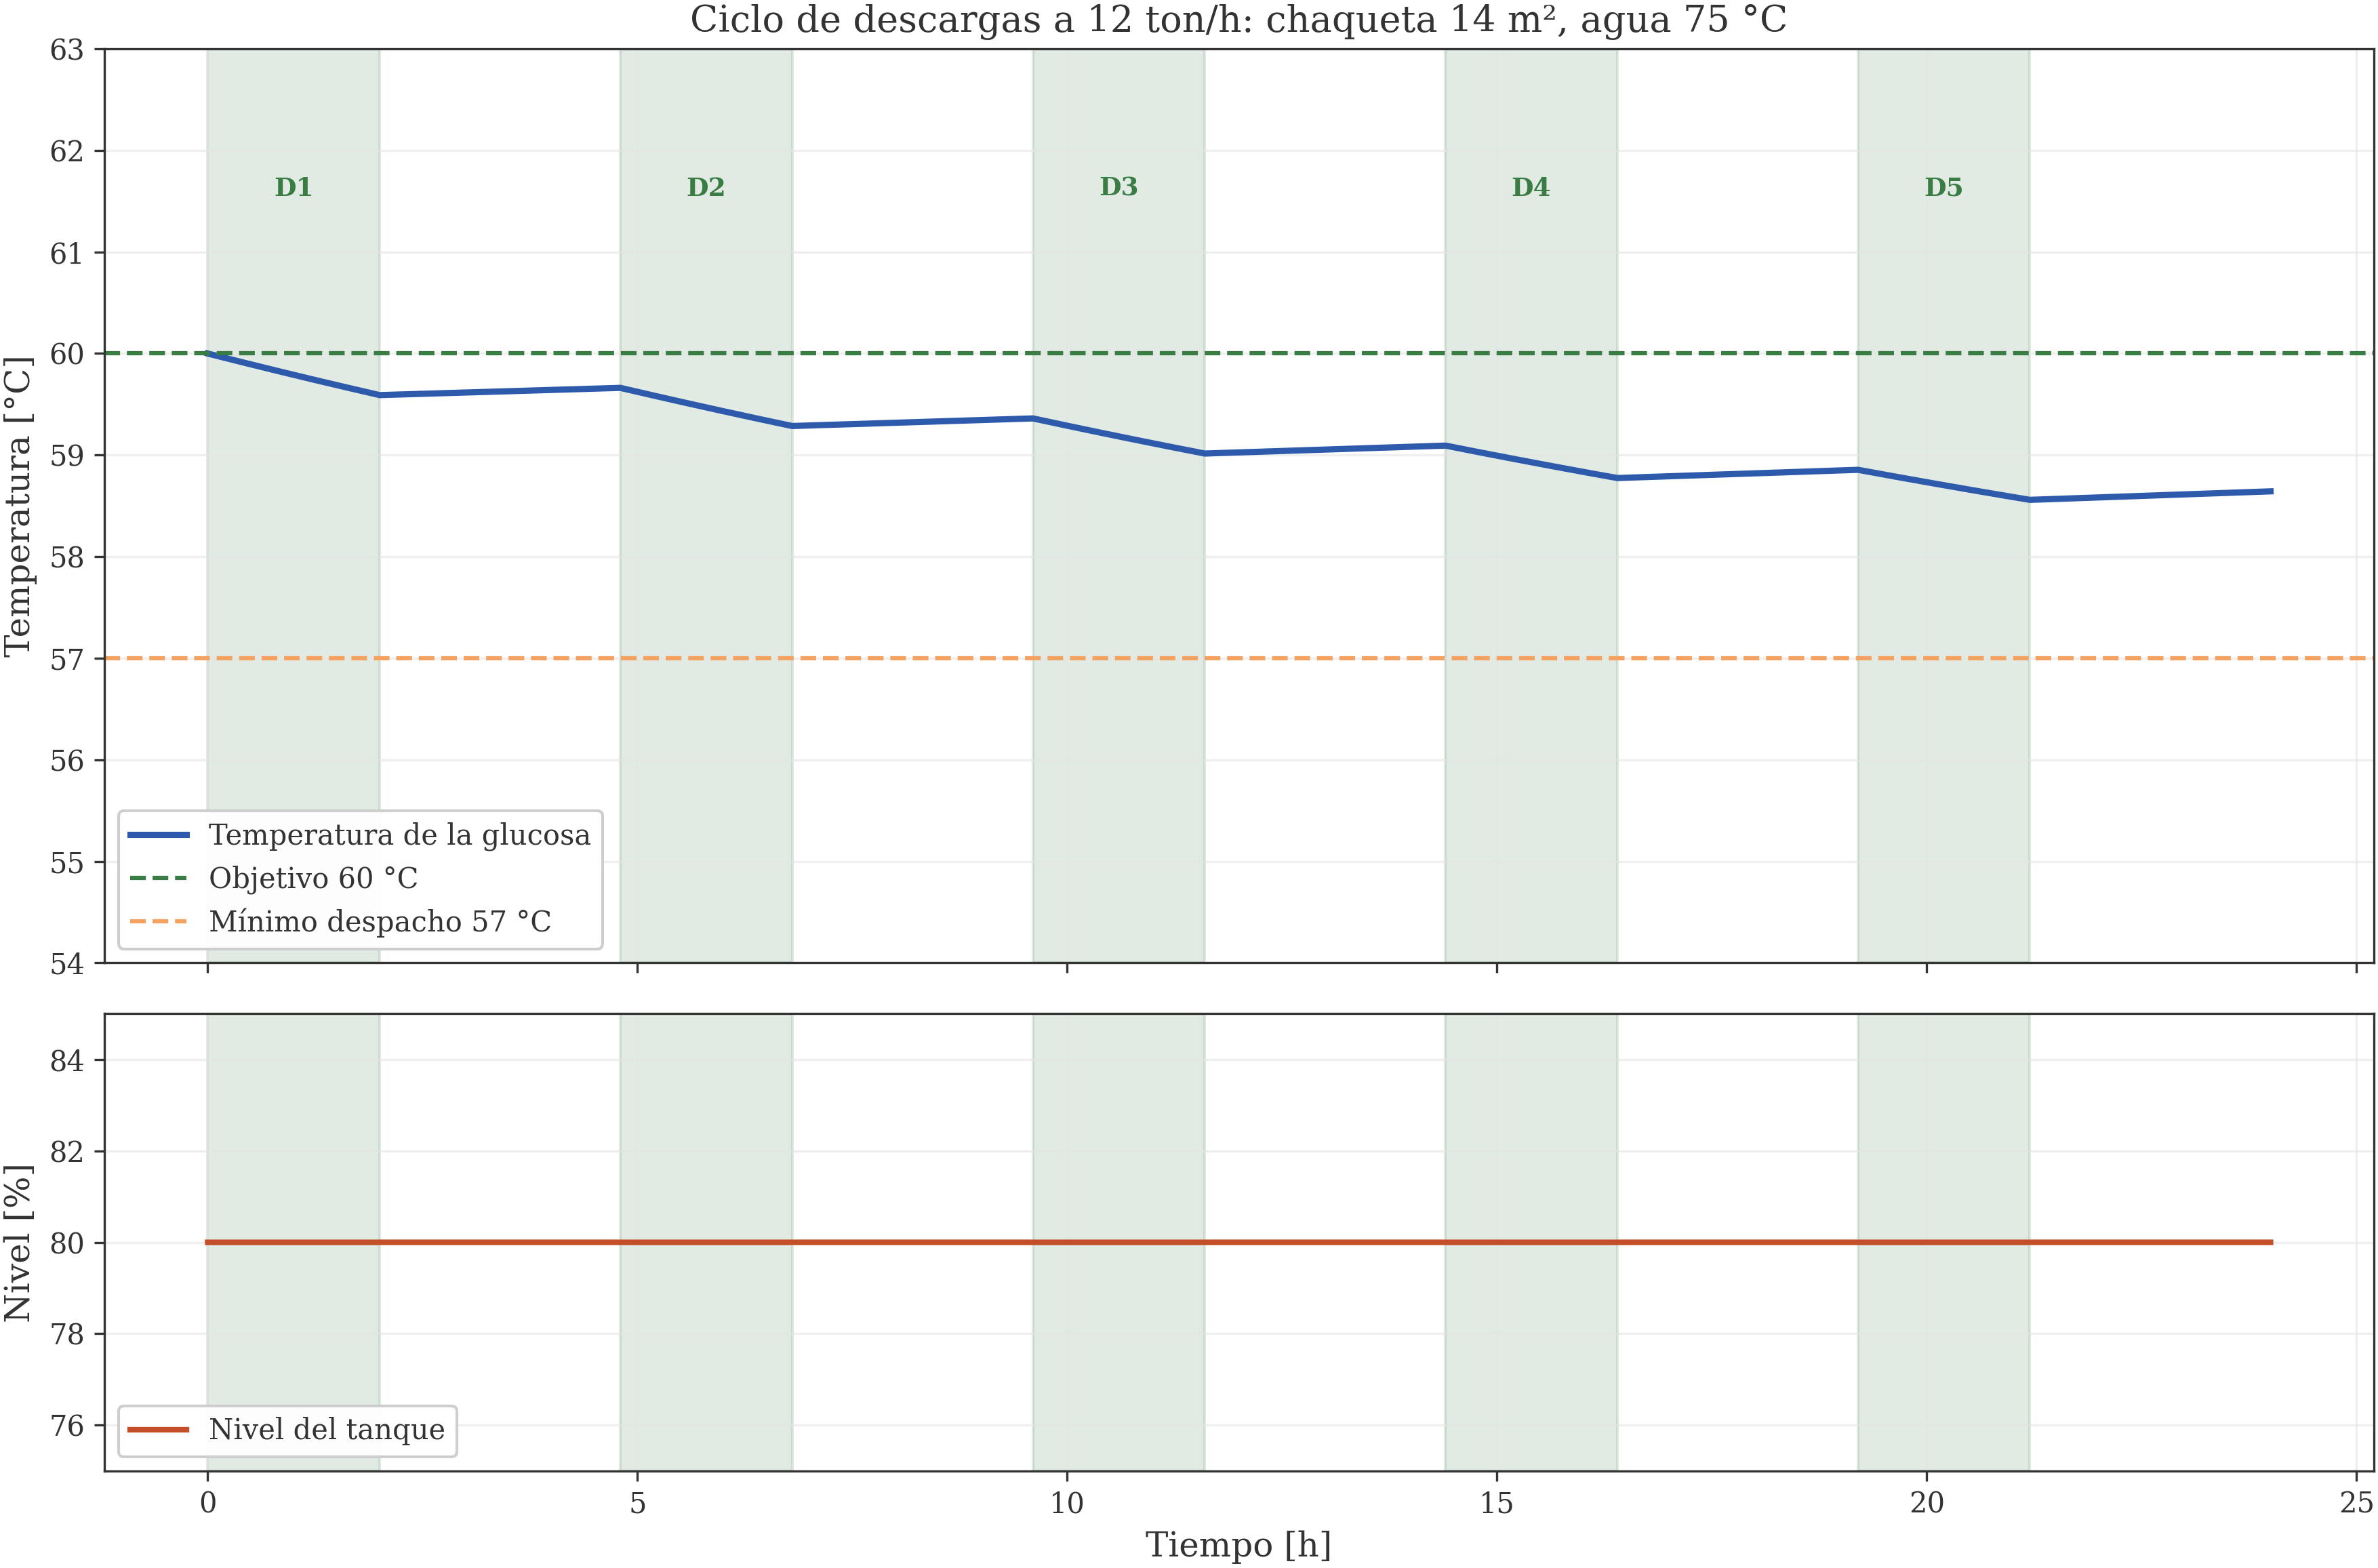
\includegraphics[width=0.95\textwidth]{../../results/figures/ciclo_12m3h_T_vs_t.pdf}
\caption{Evolución de la temperatura y del nivel del tanque durante el ciclo oficial de cinco descargas a 12~ton/h. Las bandas verdes indican los intervalos de descarga (D1 a D5).}
\label{fig:ciclo_oficial_T_vs_t}
\end{figure}

La Figura~\ref{fig:ciclo_oficial_barras_Tfin} resume la temperatura final del tanque al término de cada descarga, evidenciando que el sistema opera por encima del límite mínimo de despacho en todos los casos.

\begin{figure}[H]
\centering
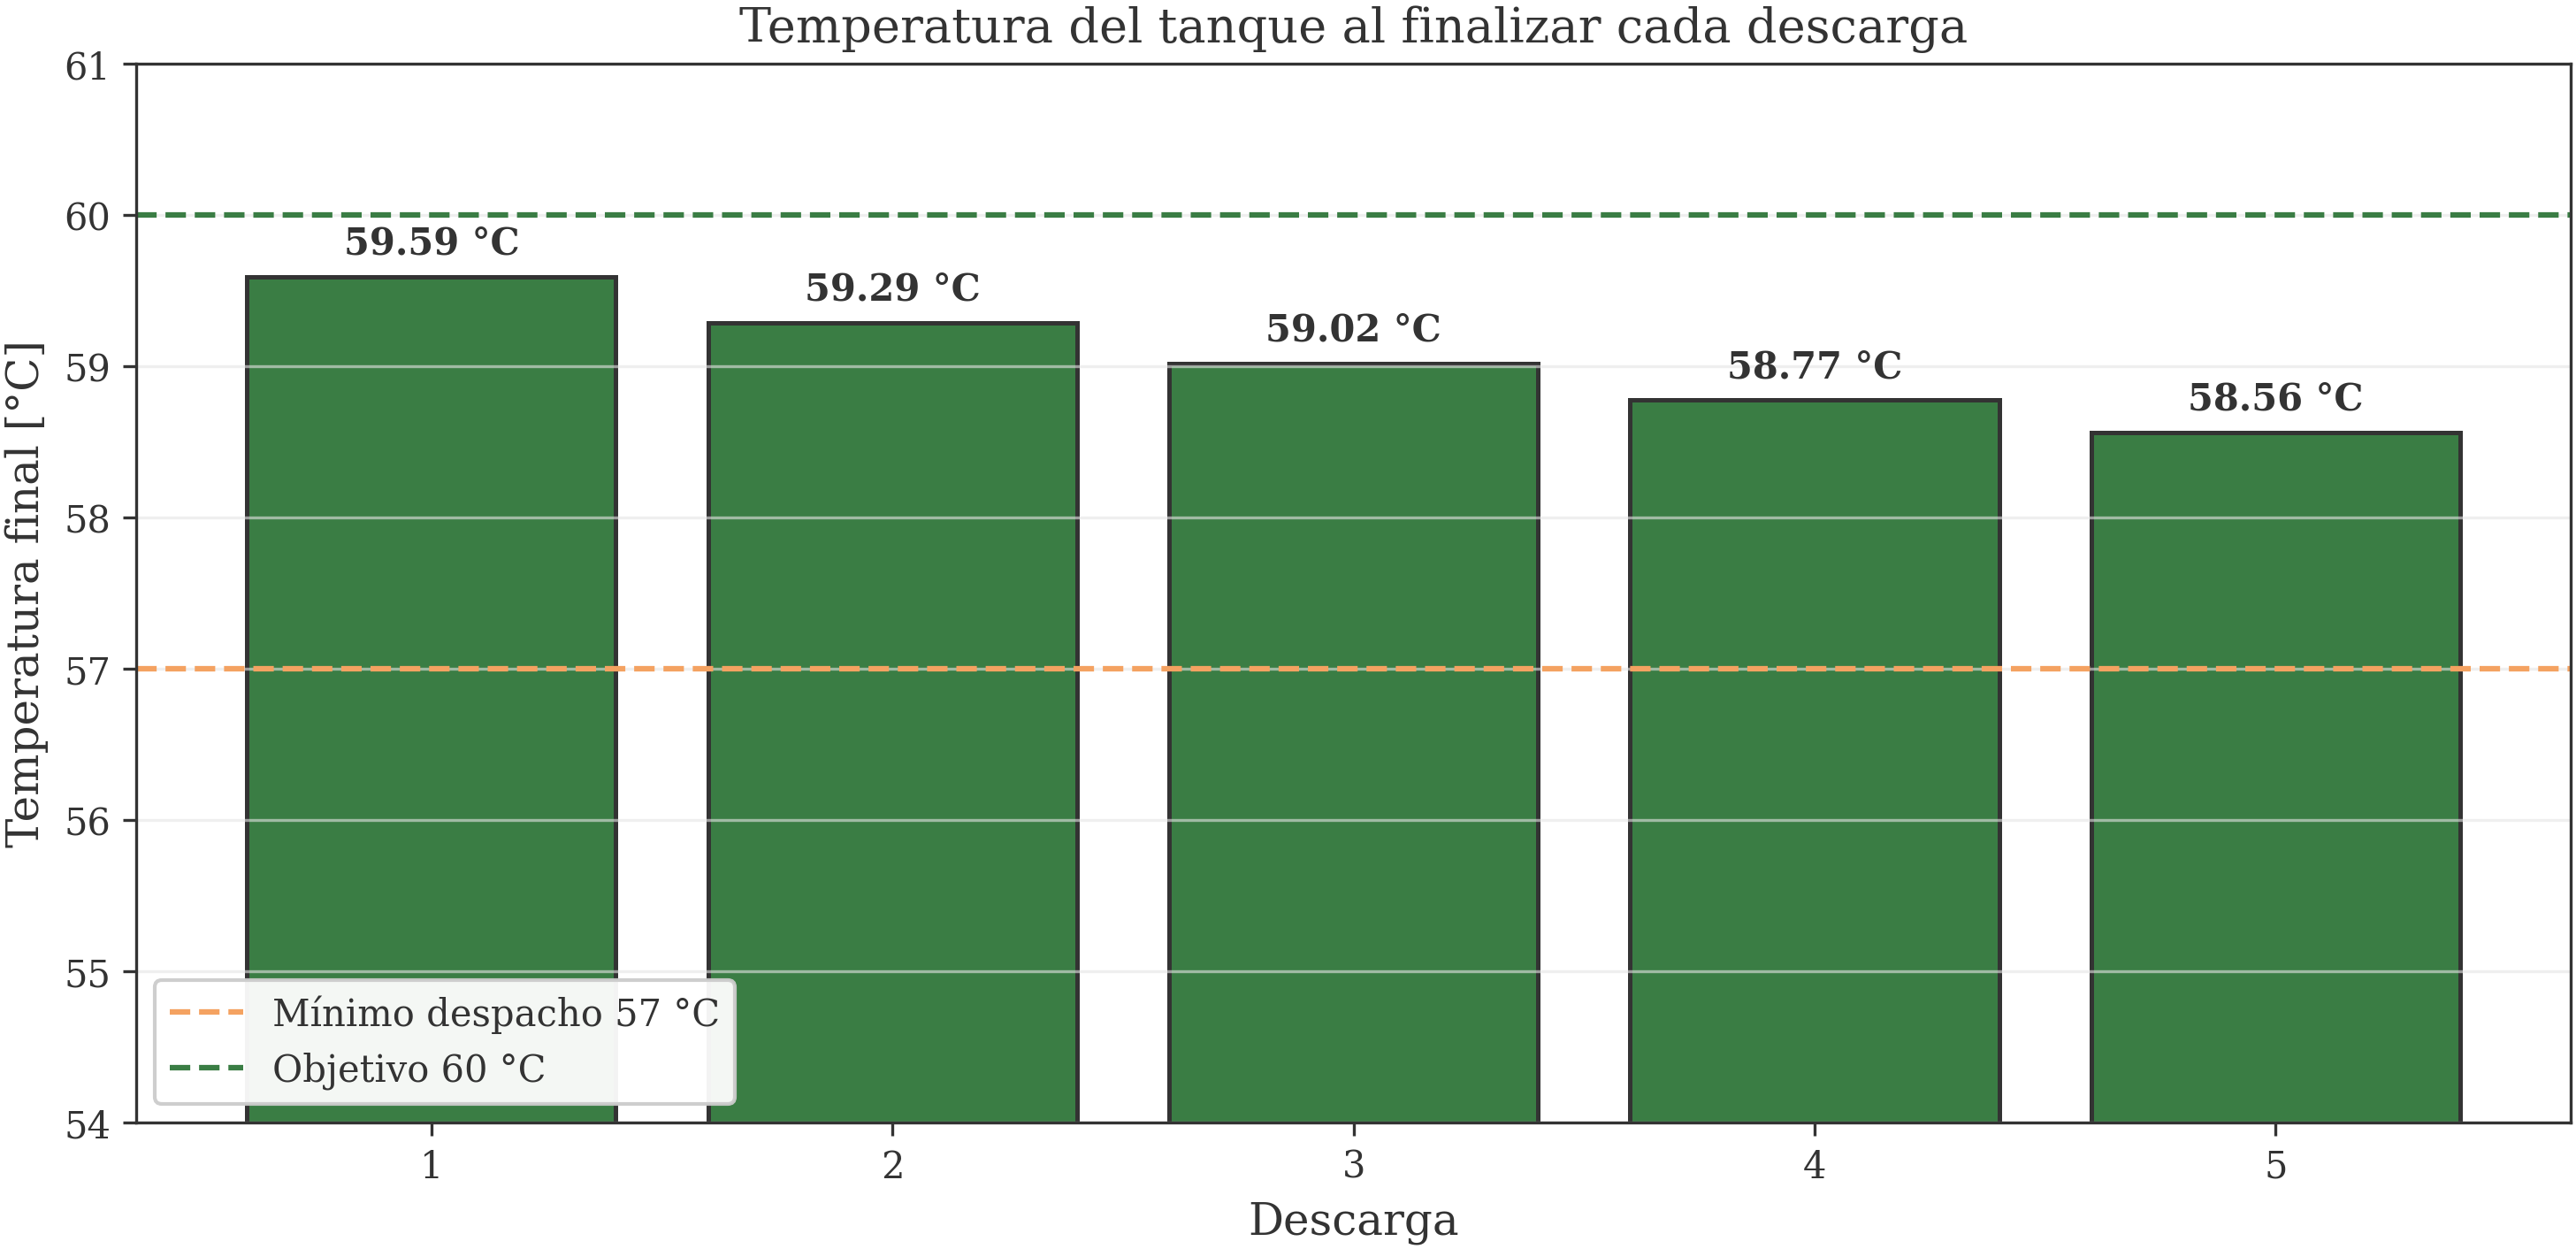
\includegraphics[width=0.85\textwidth]{../../results/figures/ciclo_12m3h_barras_Tfin.pdf}
\caption{Temperatura del tanque al finalizar cada una de las cinco descargas del ciclo oficial. La línea punteada indica el límite mínimo de despacho de 57~\textdegree C.}
\label{fig:ciclo_oficial_barras_Tfin}
\end{figure}

\subsection{Análisis paramétrico del ciclo oficial}

El ciclo oficial evaluado en la subsección anterior corresponde al caso nominal de 80~\% de nivel inicial y agua a 75~\textdegree C. Para cuantificar la sensibilidad térmica frente a dos variables críticas ---temperatura del agua de calentamiento y nivel inicial del tanque--- se ejecutaron cuatro escenarios paramétricos conservando el flujo de descarga de 12~ton/h, el área de 14~m\textsuperscript{2} y las pérdidas térmicas reales.

\begin{table}[H]
\centering
\caption{Comparación paramétrica del ciclo de cinco descargas diarias con pérdidas térmicas reales.}
\label{tab:comparacion_parametrica_ciclo}
\begin{tabular}{@{}lcccc@{}}
\toprule
\textbf{Escenario} & \textbf{Nivel inicial} & \textbf{$T_w$ [\textdegree C]} & \textbf{$T_{min}$ [\textdegree C]} & \textbf{Factible ($T \geq 57$~\textdegree C)} \\
\midrule
Base & 80~\% & 75 & 58,56 & Sí \\
G & 80~\% & 65 & 57,88 & Sí \\
H & 50~\% & 75 & 58,01 & Sí \\
I & 50~\% & 65 & 57,08 & Sí \\
\bottomrule
\end{tabular}
\end{table}

Todos los escenarios cumplen el criterio mínimo de despacho de 57~\textdegree C. Sin embargo, el margen de seguridad se reduce conforme disminuye el nivel inicial o la temperatura del agua. El escenario más crítico (50~\% y 65~\textdegree C) termina la quinta descarga a 57,11~\textdegree C, apenas 0,11~\textdegree C por encima del límite. En todos los casos con agua a 65~\textdegree C, el tiempo muerto entre descargas presenta una ganancia térmica neta negativa, es decir, las pérdidas al ambiente superan el aporte de la chaqueta durante la recuperación; la temperatura sigue cayendo, aunque lo hace lentamente gracias a la inercia térmica del contenido.

La Figura~\ref{fig:ciclo_parametrico_80pct} compara el perfil de temperatura para el nivel inicial de 80~\% con agua a 65~\textdegree C y 75~\textdegree C. La Figura~\ref{fig:ciclo_parametrico_50pct} presenta el mismo análisis para el 50~\% de nivel inicial.

\begin{figure}[H]
\centering
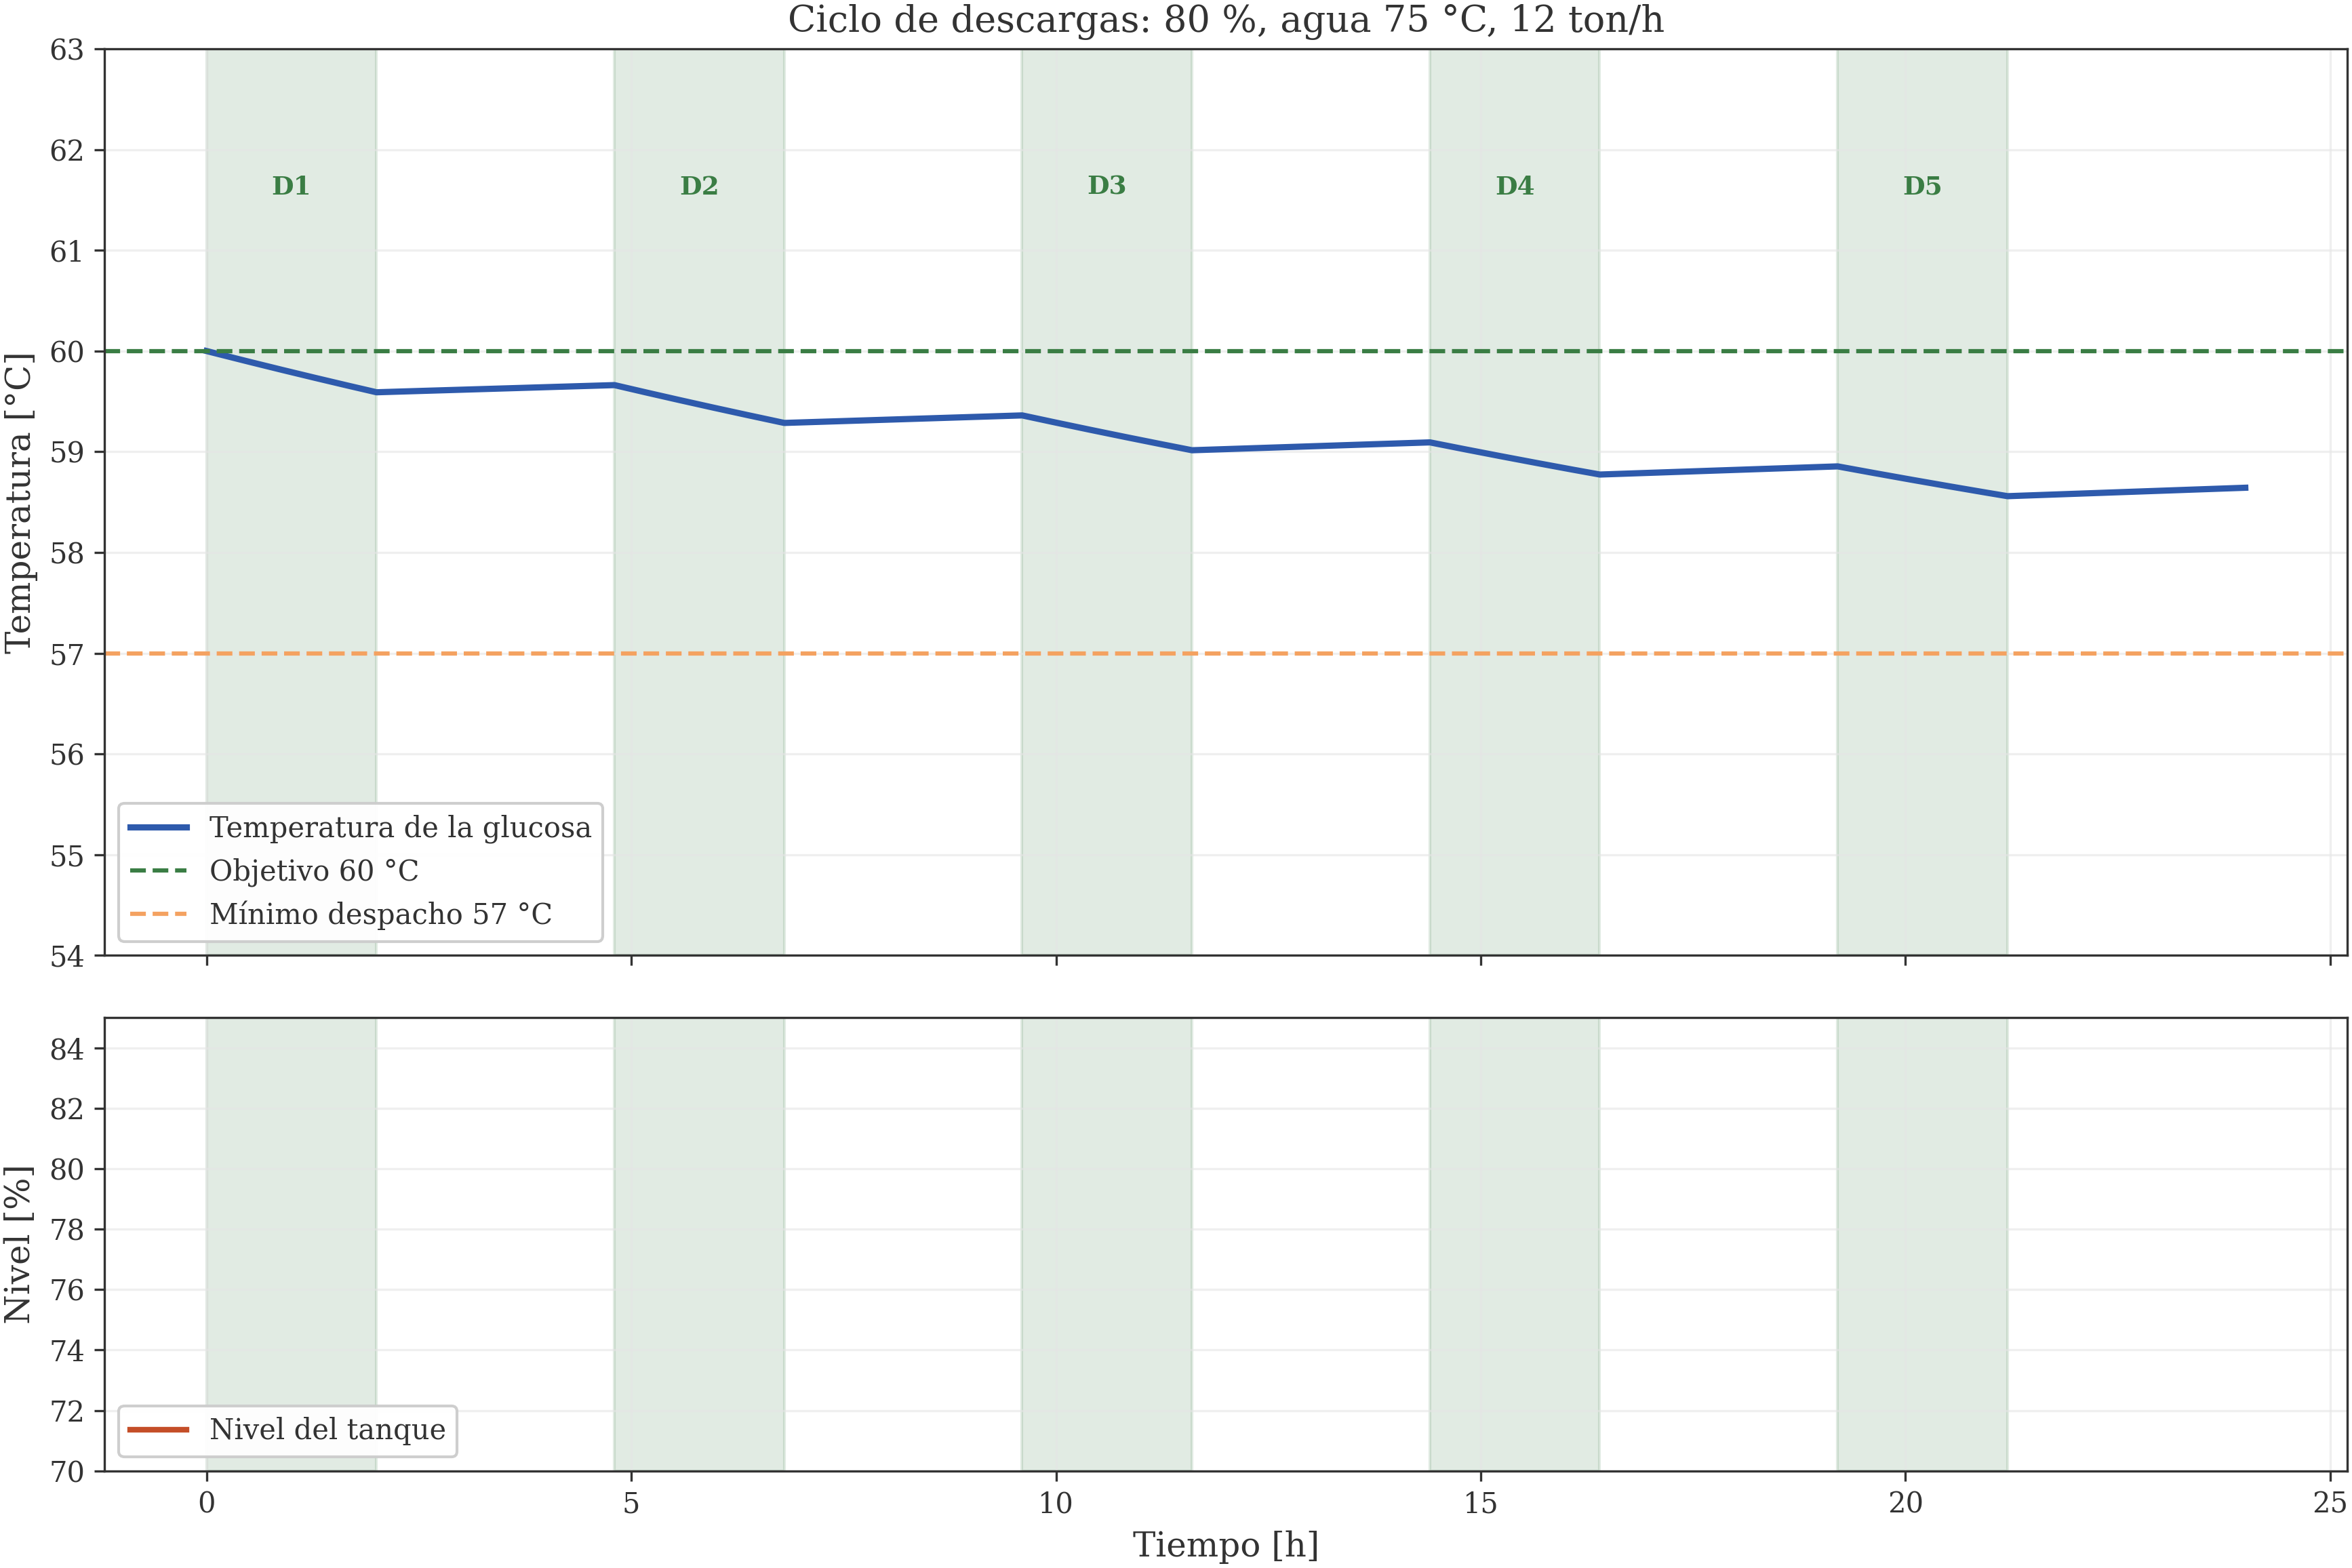
\includegraphics[width=0.48\textwidth]{../../results/figures/ciclo_80pct_75C_T_vs_t.pdf}
\hfill
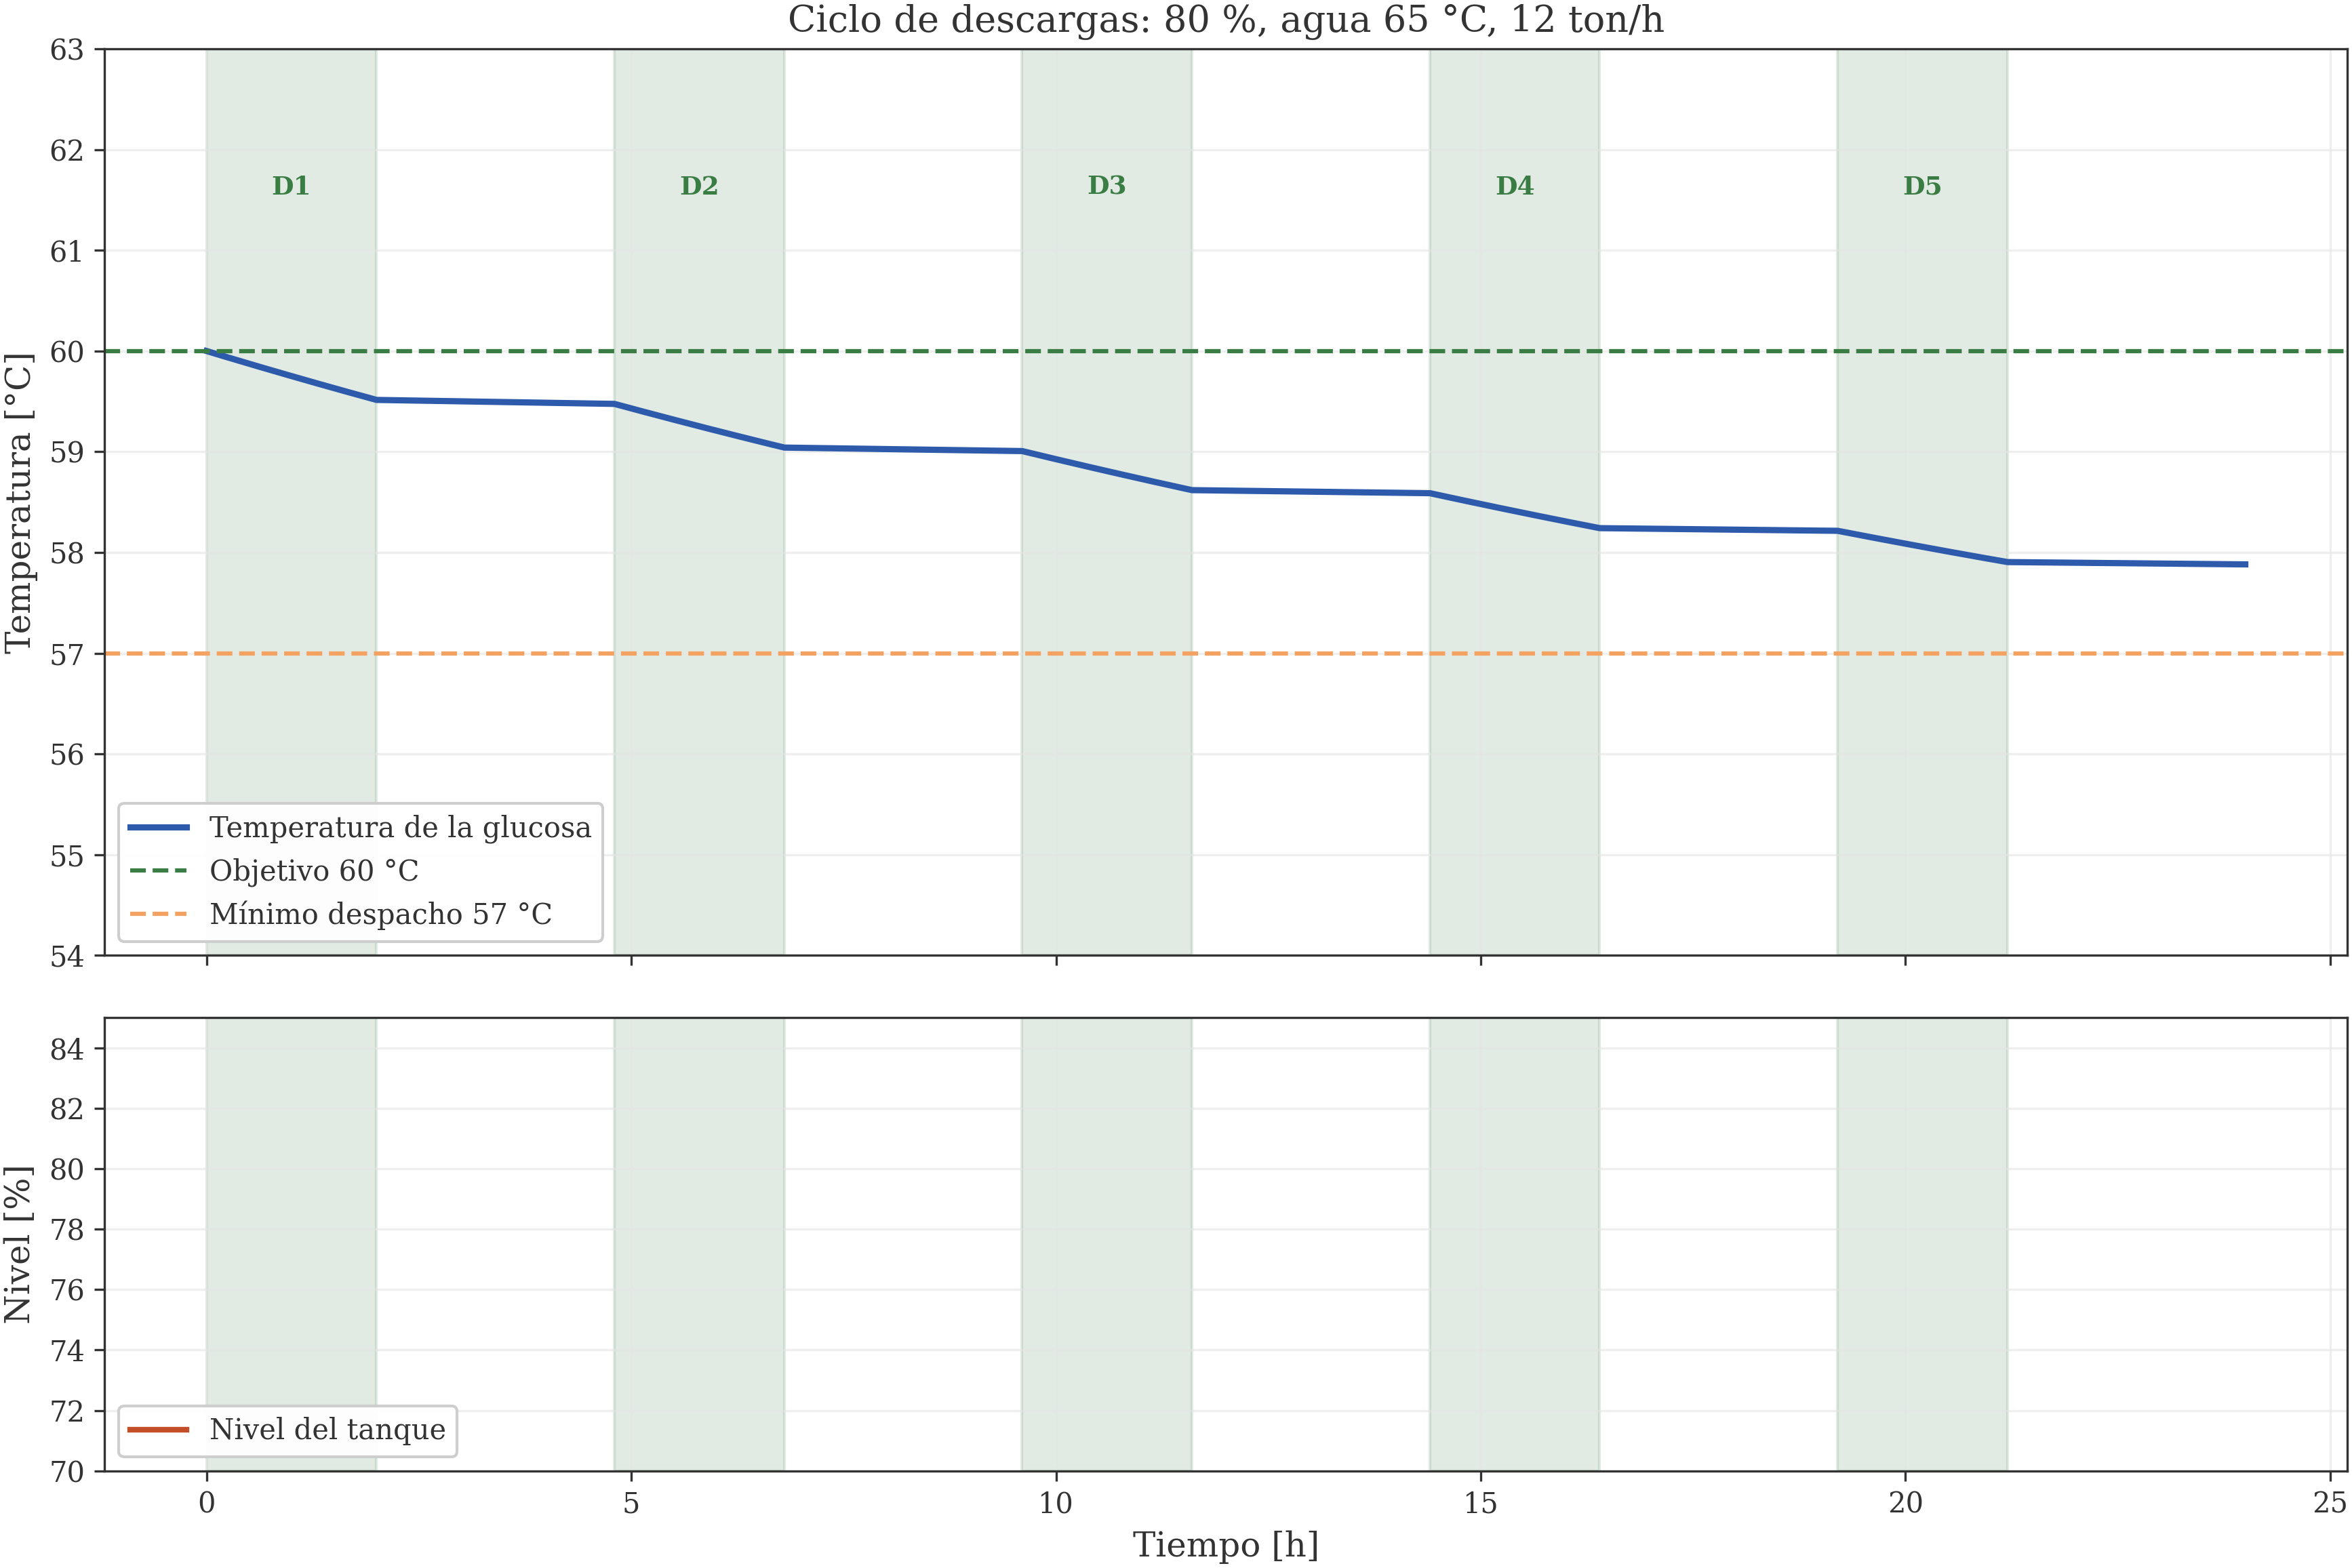
\includegraphics[width=0.48\textwidth]{../../results/figures/ciclo_80pct_65C_T_vs_t.pdf}
\caption{Perfil de temperatura del ciclo oficial con nivel inicial de 80~\%: (izquierda) agua a 75~\textdegree C; (derecha) agua a 65~\textdegree C. Las bandas verdes indican los intervalos de descarga.}
\label{fig:ciclo_parametrico_80pct}
\end{figure}

\begin{figure}[H]
\centering
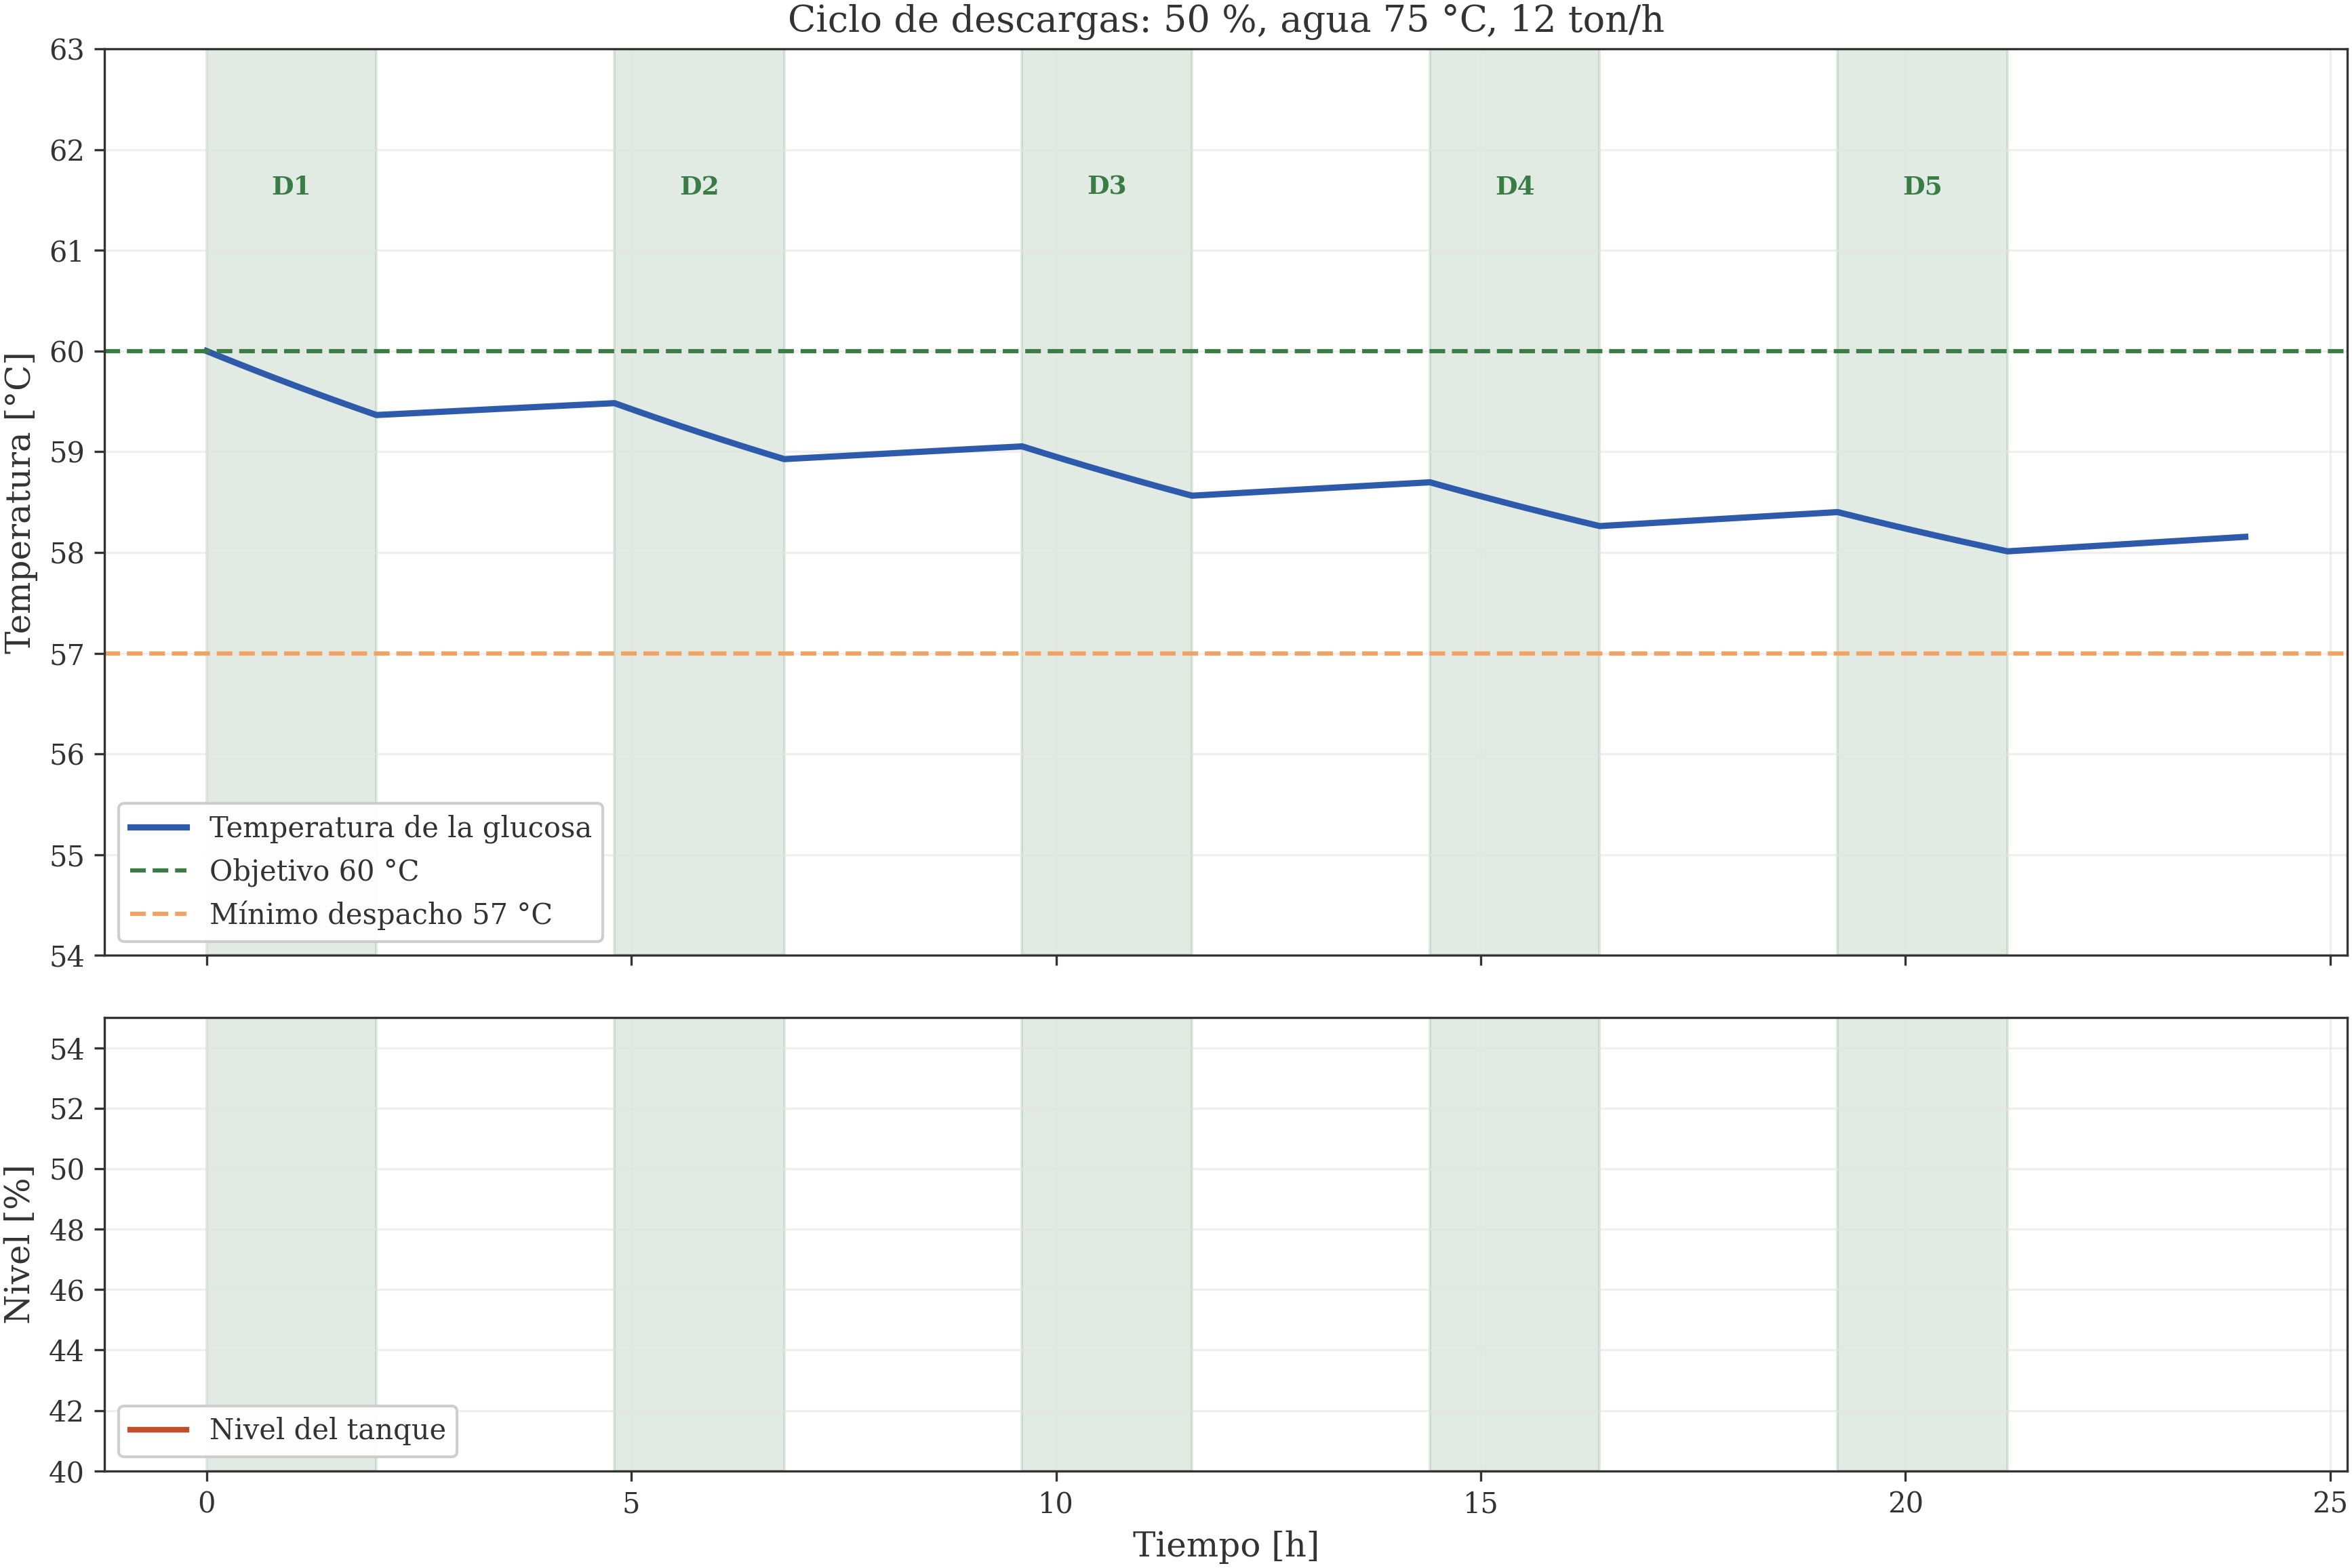
\includegraphics[width=0.48\textwidth]{../../results/figures/ciclo_50pct_75C_T_vs_t.pdf}
\hfill
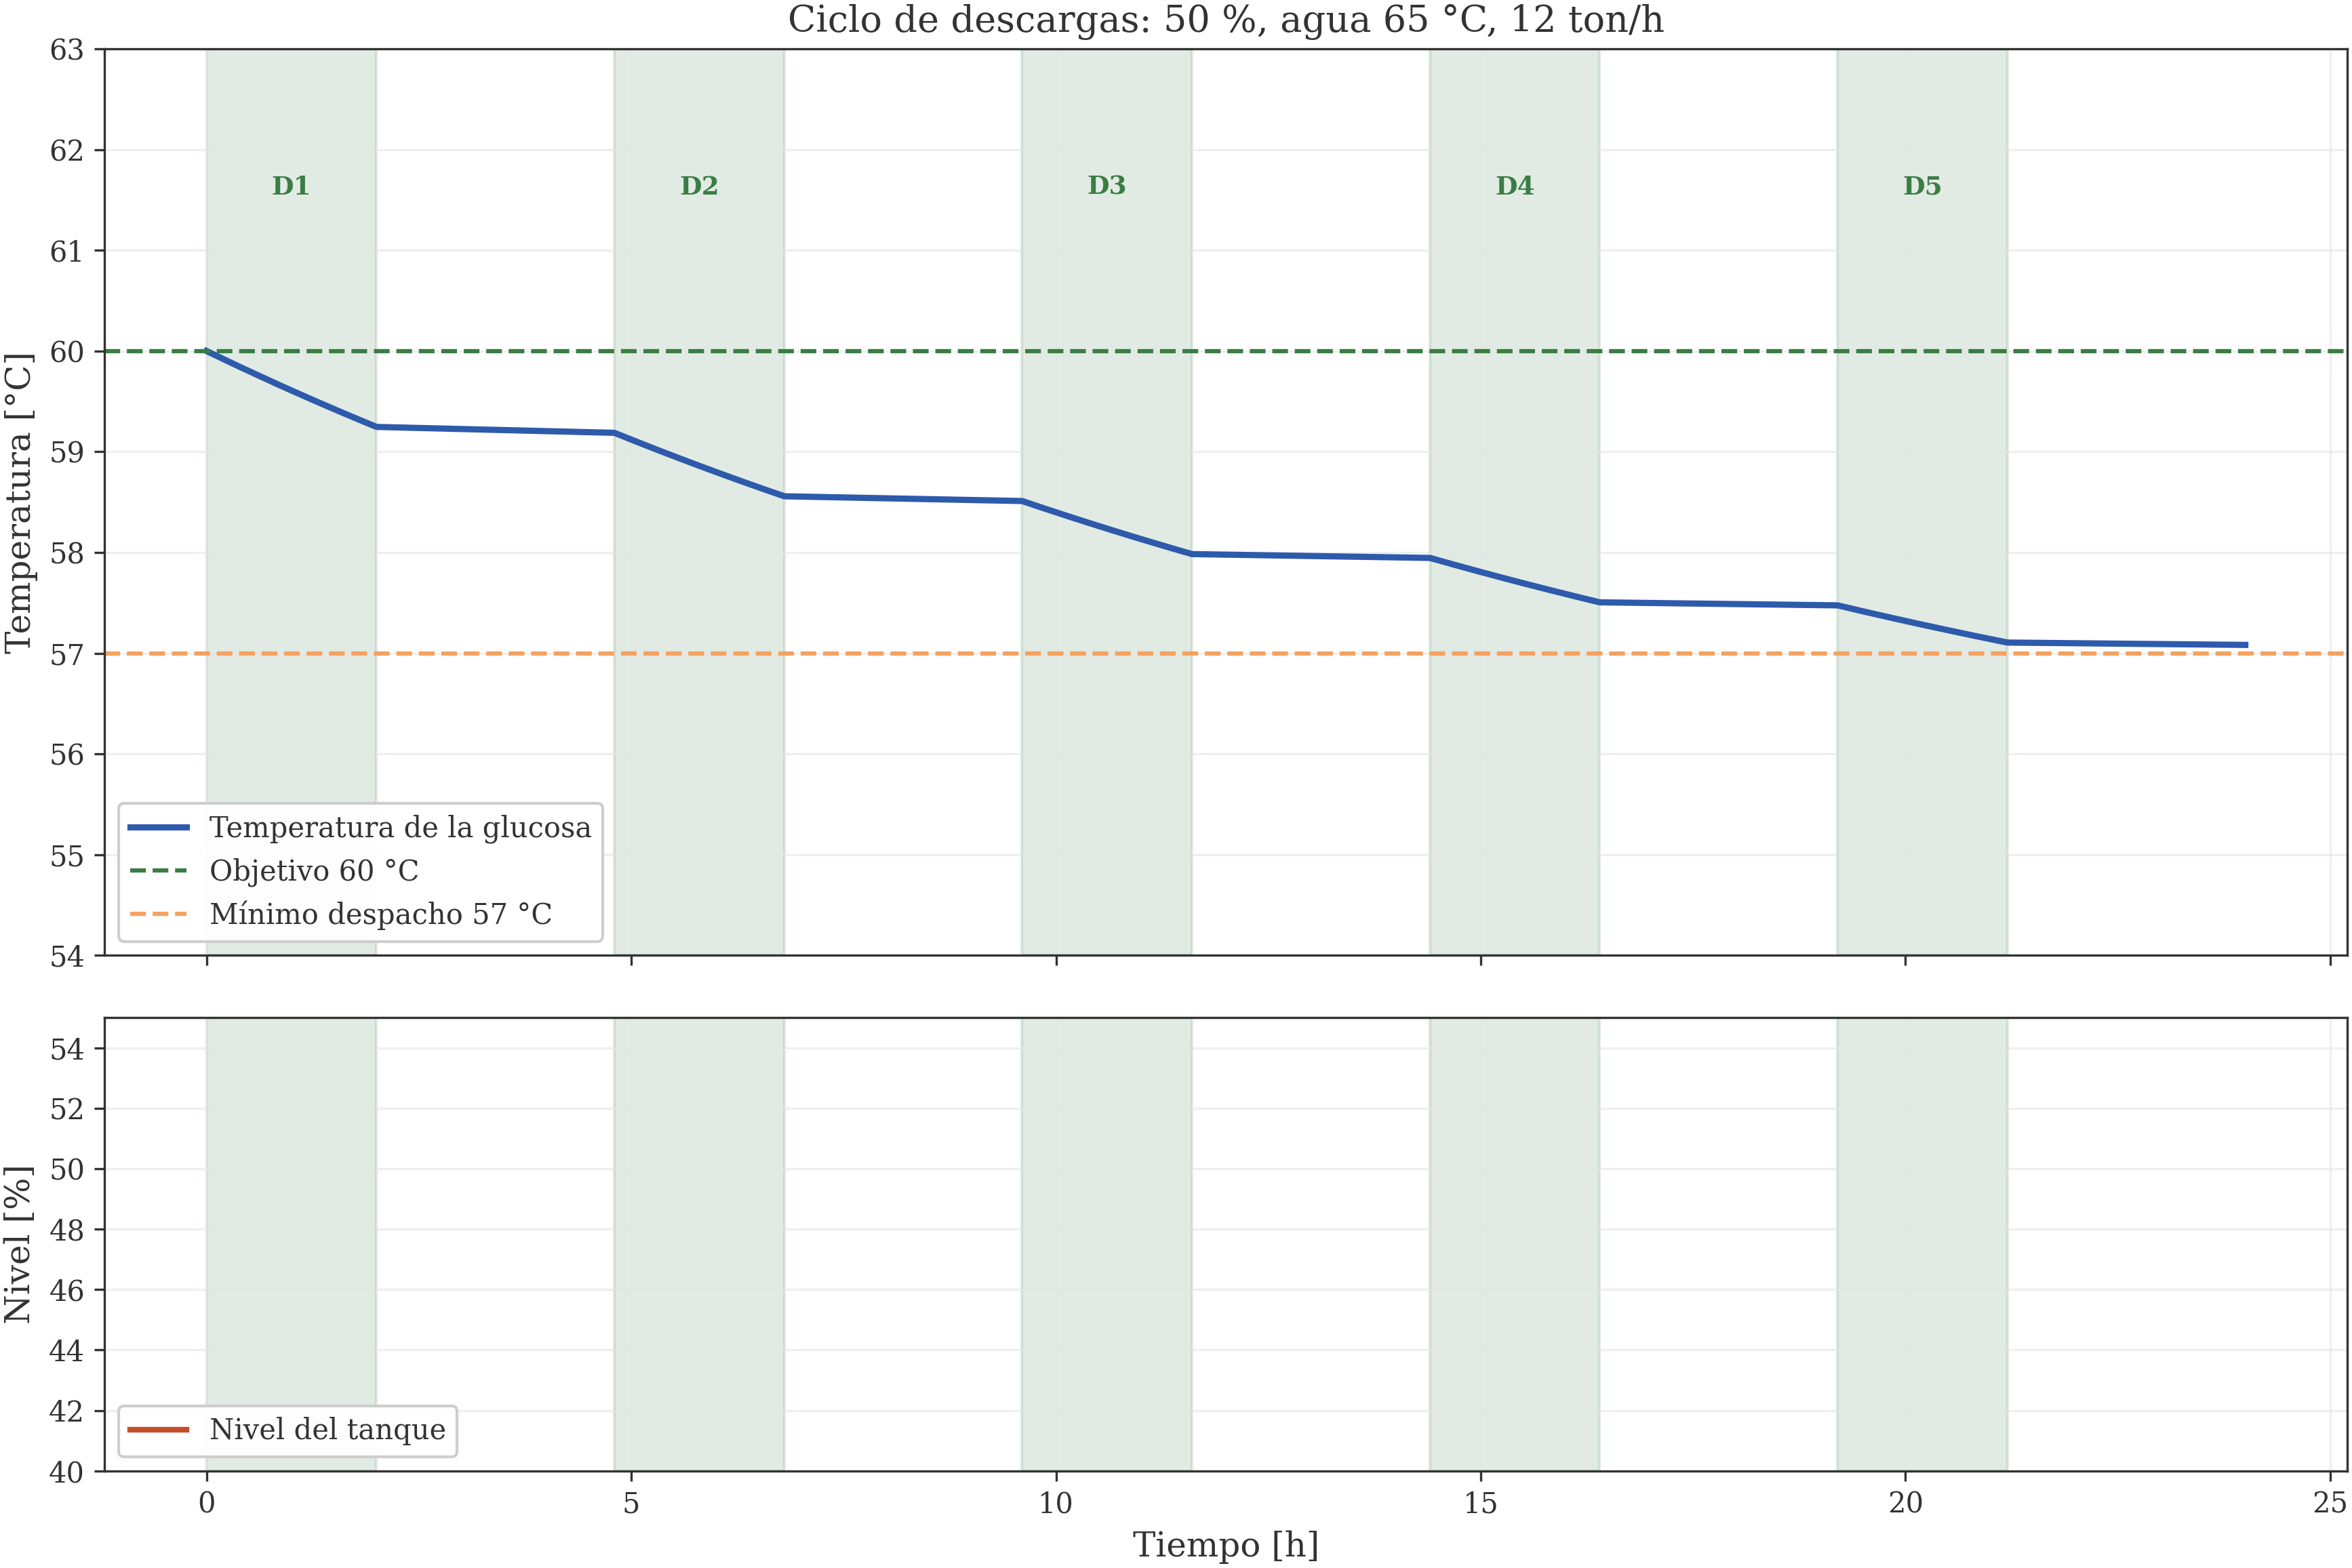
\includegraphics[width=0.48\textwidth]{../../results/figures/ciclo_50pct_65C_T_vs_t.pdf}
\caption{Perfil de temperatura del ciclo oficial con nivel inicial de 50~\%: (izquierda) agua a 75~\textdegree C; (derecha) agua a 65~\textdegree C.}
\label{fig:ciclo_parametrico_50pct}
\end{figure}

La caída de temperatura entre descargas es mayor cuando el nivel inicial es menor, porque la masa térmica disponible es menor y la misma entrada de glucosa a 55~\textdegree C representa una fracción más significativa del contenido total. Asimismo, con agua a 65~\textdegree C la recuperación entre descargas es insuficiente para compensar el enfriamiento, por lo que el sistema converge hacia un estado pseudoestacionario por debajo de 60~\textdegree C.

\subsection{Diagramas de flujo de bloques del ciclo}

La Figura~\ref{fig:diagrama_bloques_descarga} representa el balance de masa y energía durante la fase de descarga. La glucosa de alimentación ingresa a 55~\textdegree C mientras la chaqueta aporta calor y se compensan las pérdidas al ambiente; simultáneamente, el producto caliente se dirige al carrotanque.

\begin{figure}[H]
\centering
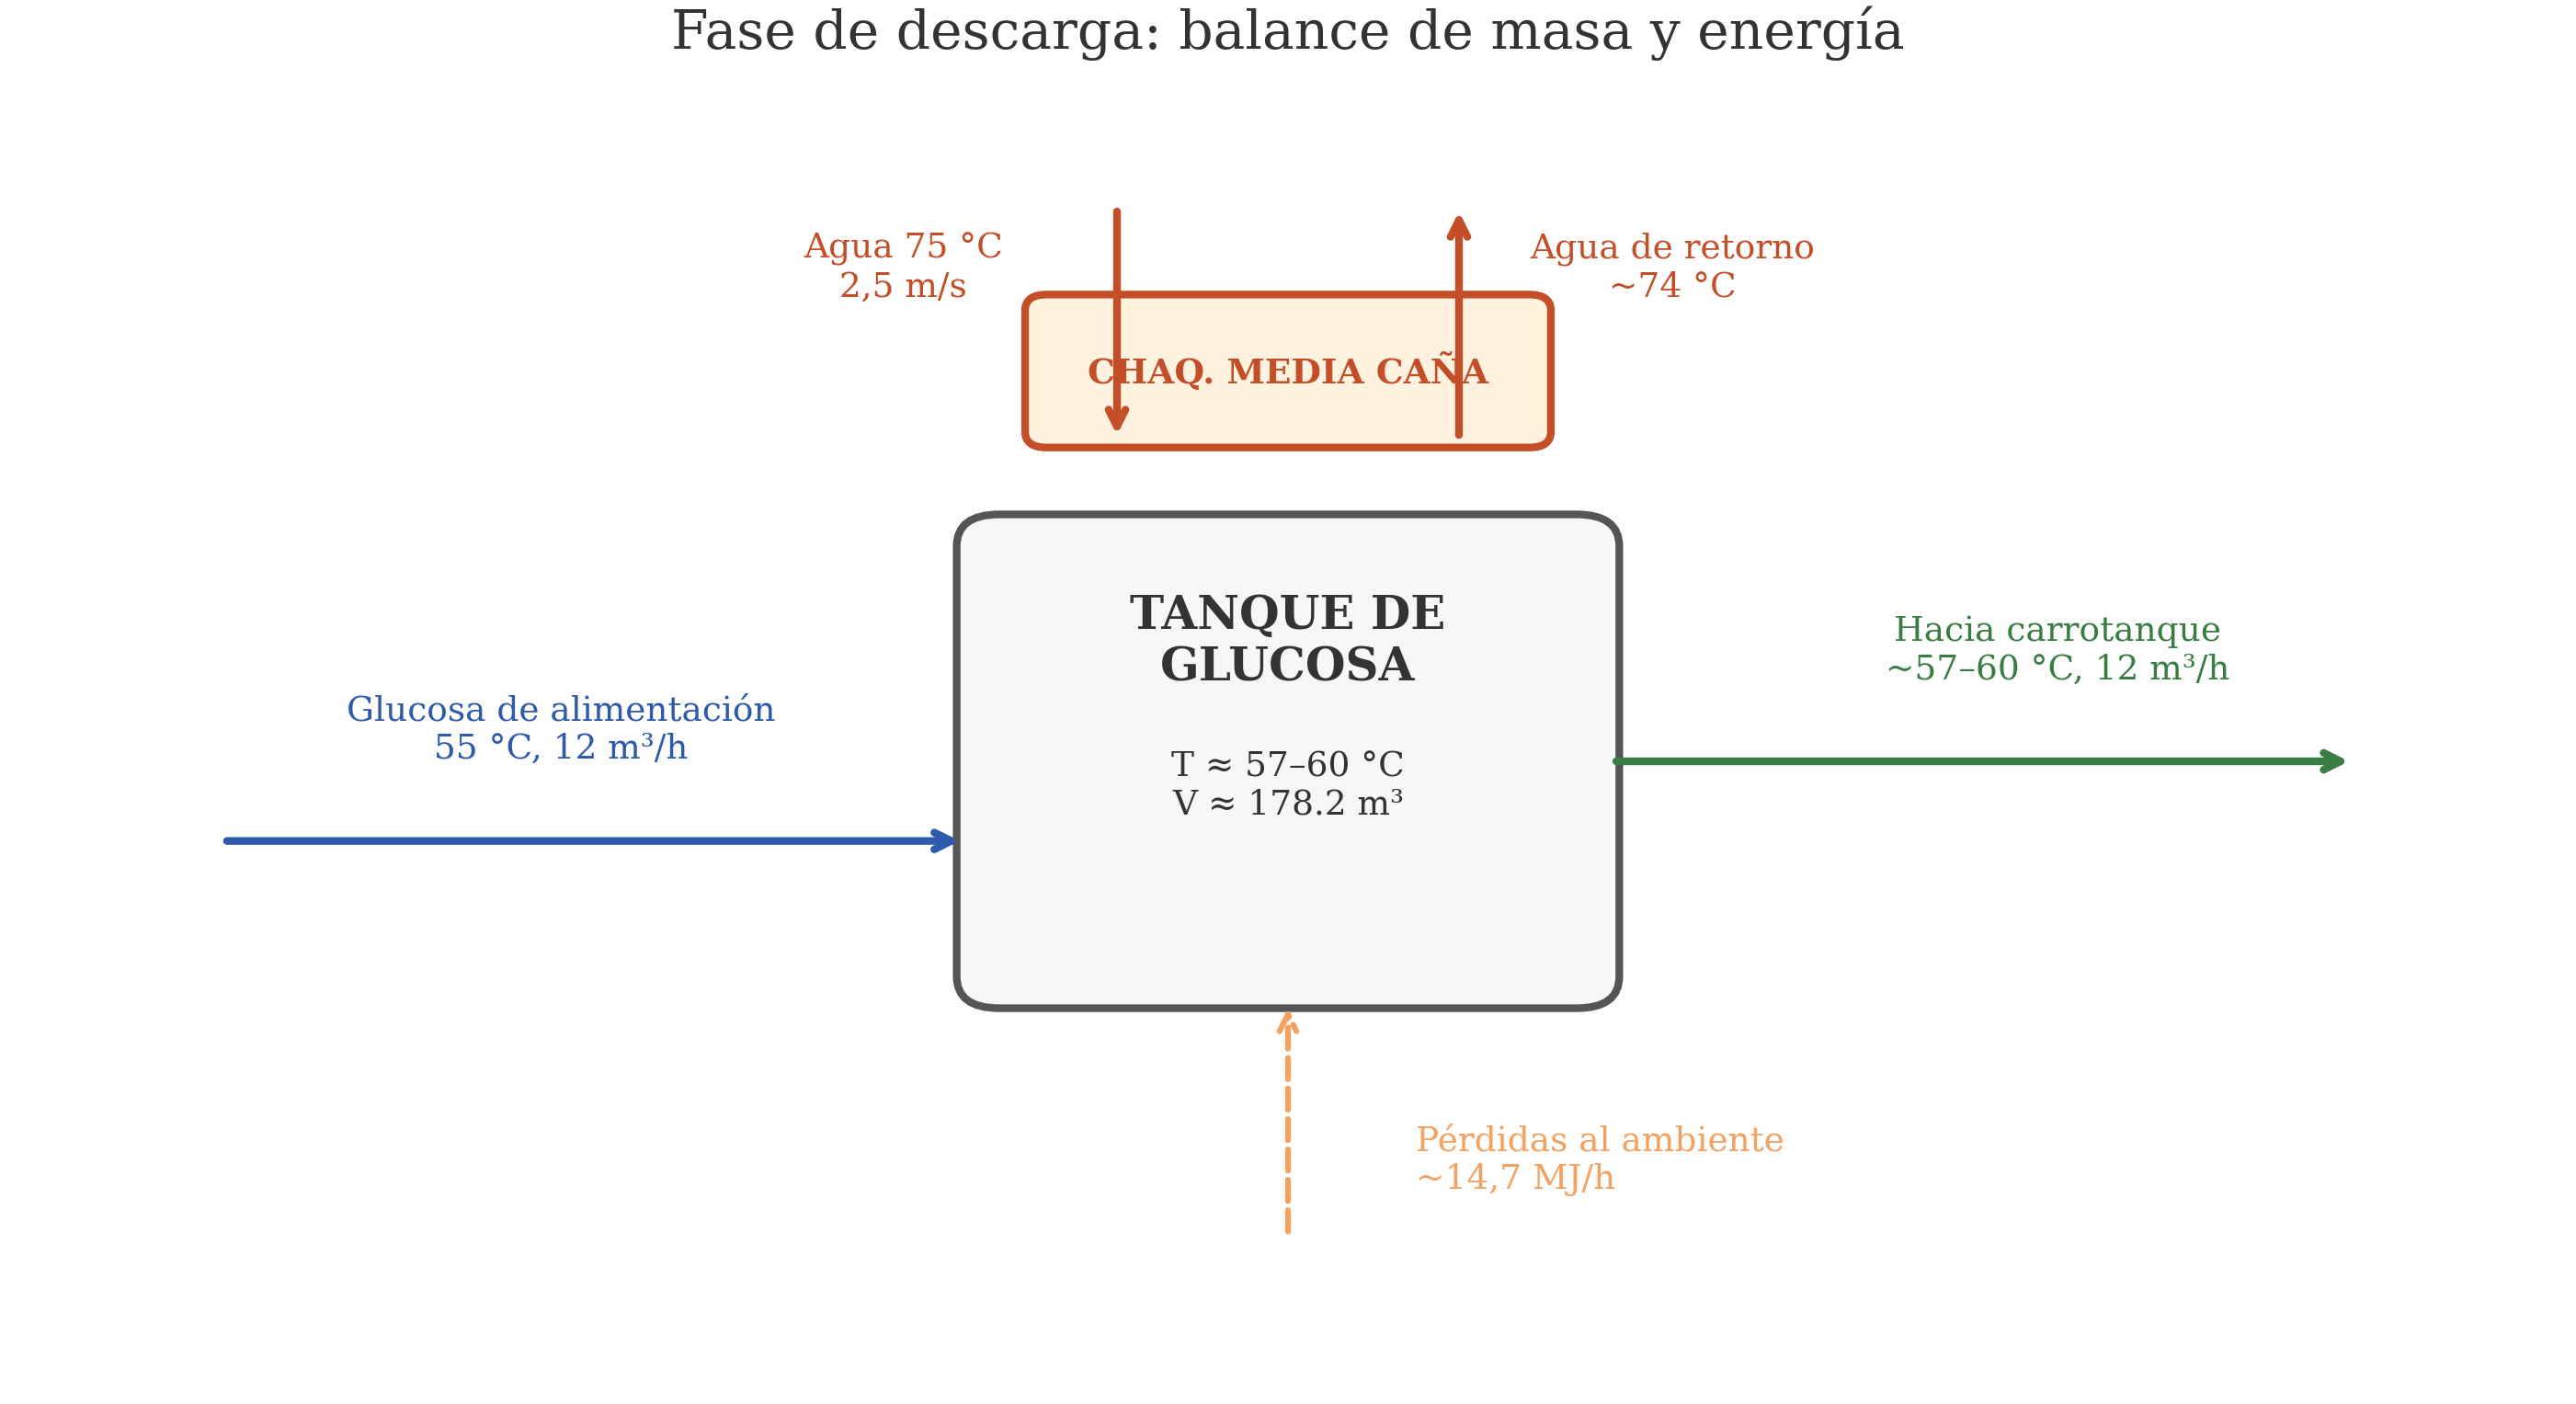
\includegraphics[width=0.95\textwidth]{../../results/figures/diagrama_bloques_descarga.pdf}
\caption{Diagrama de bloques de la fase de descarga: entrada de glucosa fría, aporte térmico de la chaqueta, pérdidas al ambiente y salida hacia el carrotanque.}
\label{fig:diagrama_bloques_descarga}
\end{figure}

La Figura~\ref{fig:diagrama_bloques_calentamiento} ilustra la fase de recuperación de temperatura entre descargas, en la cual el tanque no tiene flujo de entrada ni salida y la chaqueta eleva la temperatura compensando las pérdidas térmicas.

\begin{figure}[H]
\centering
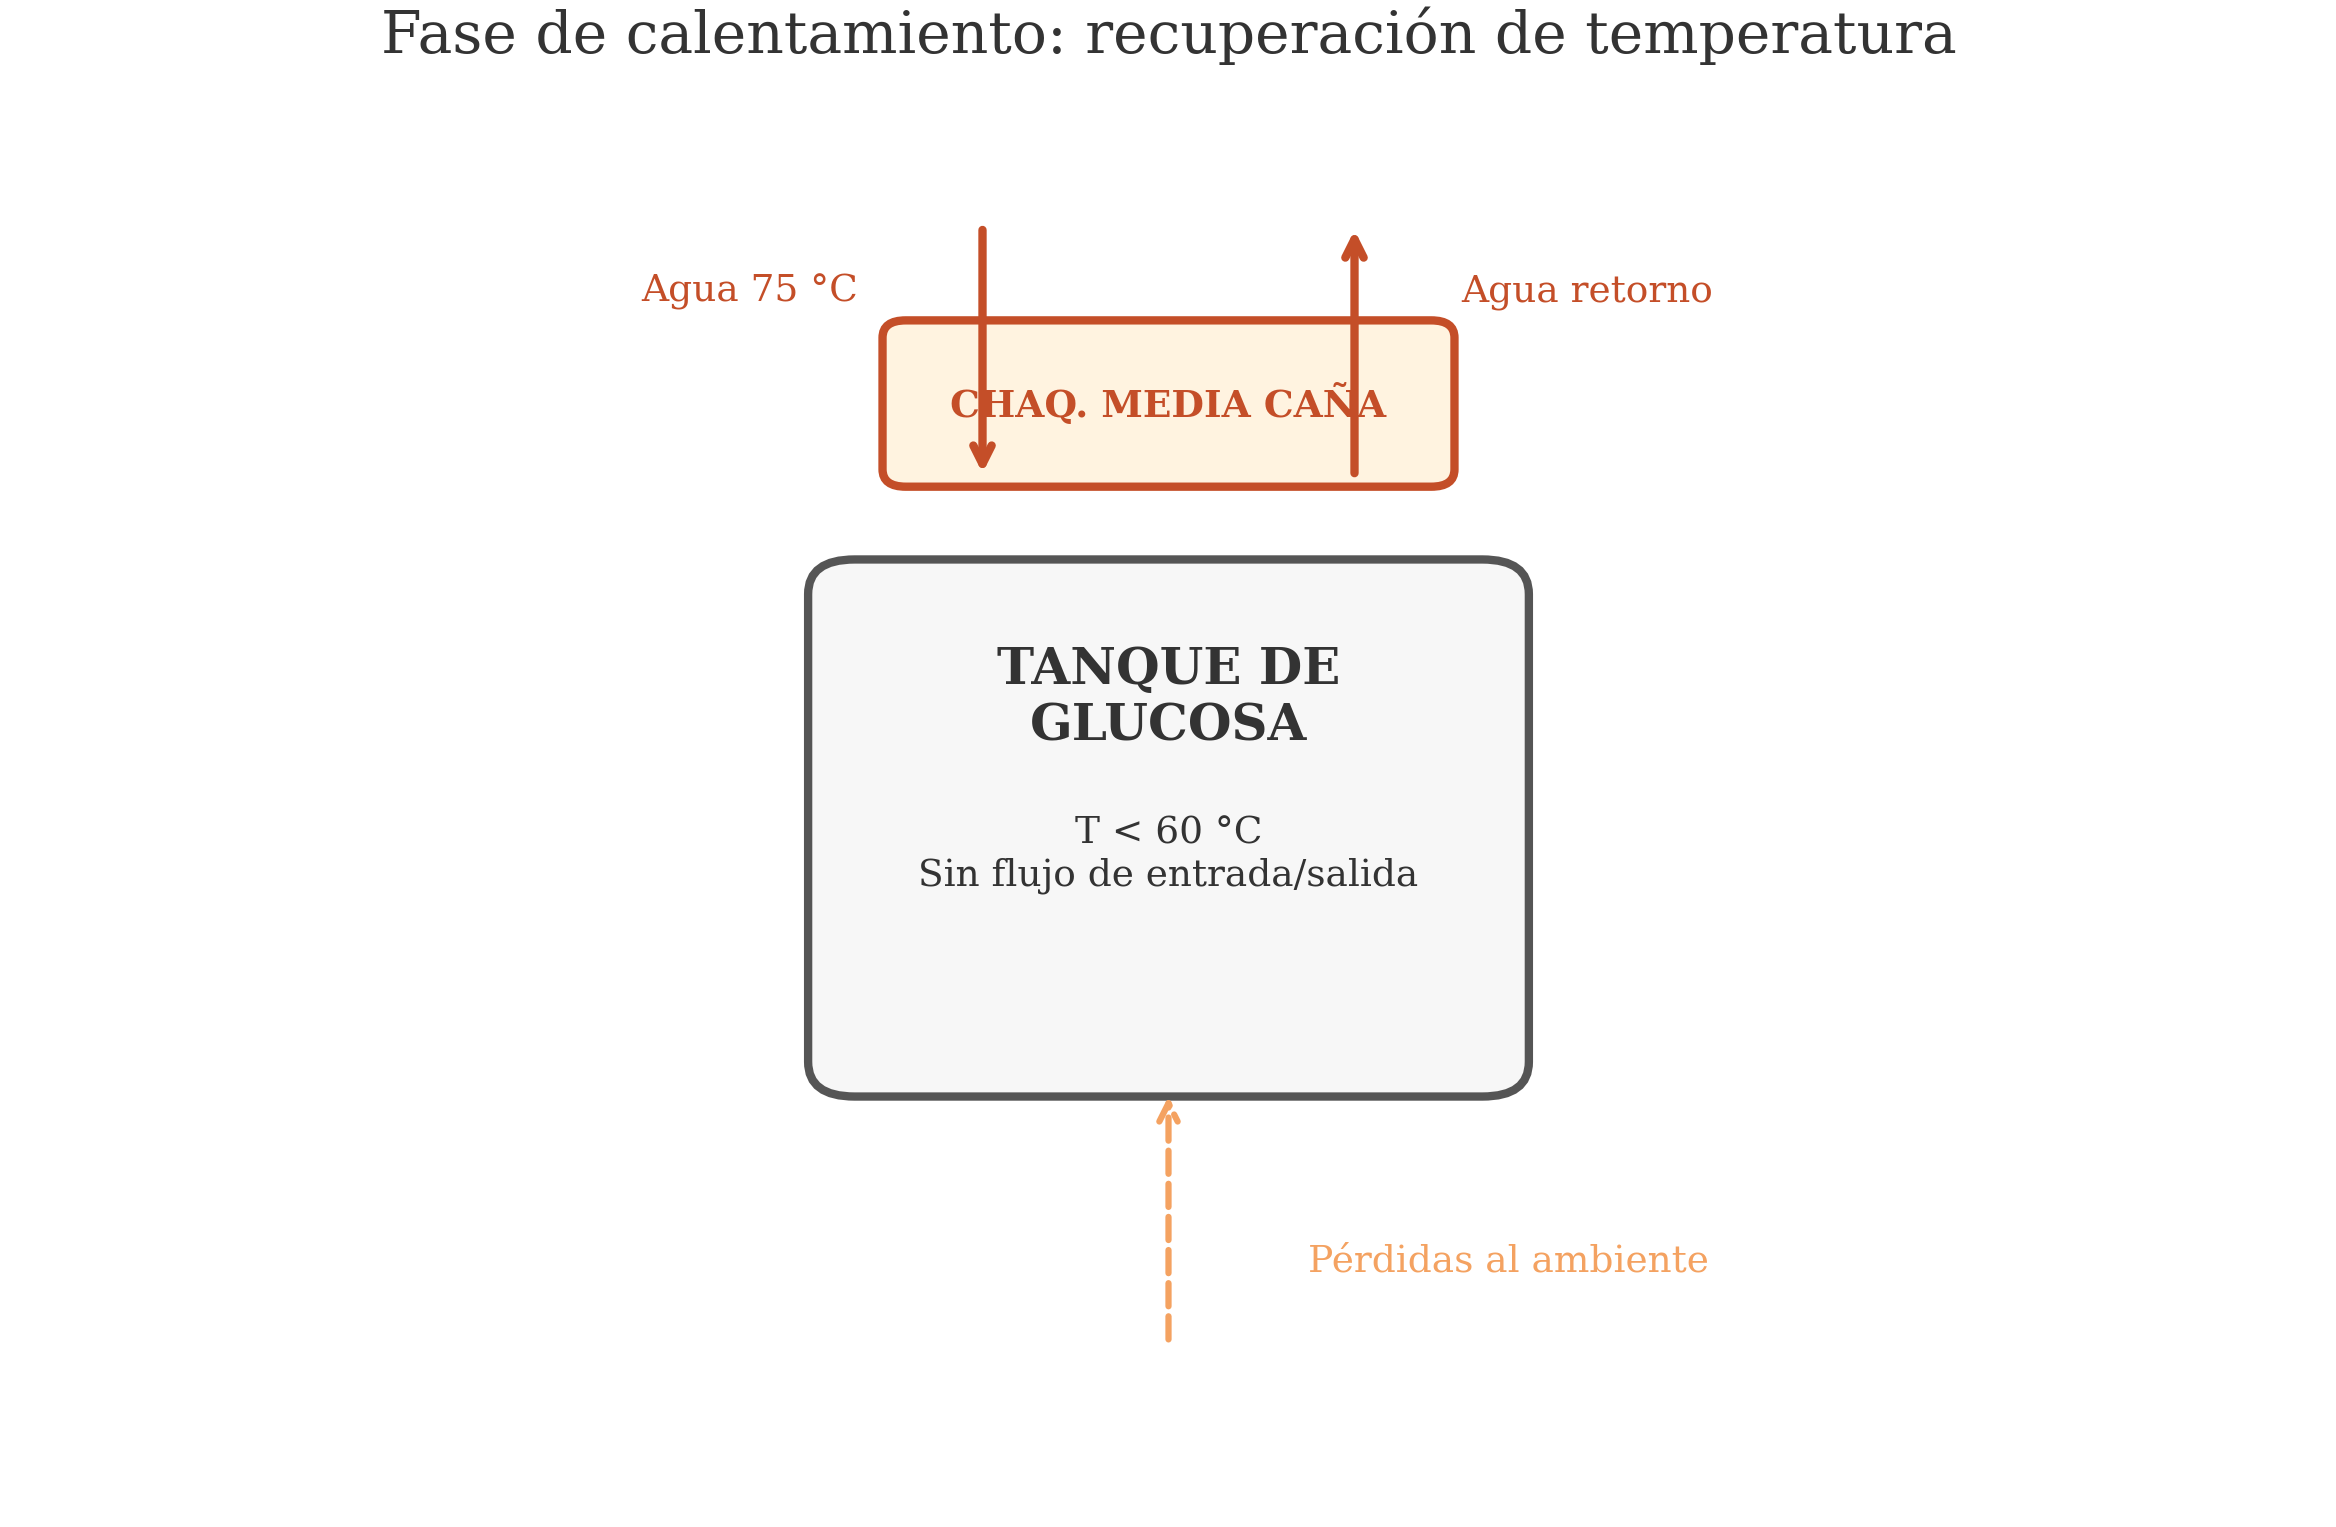
\includegraphics[width=0.85\textwidth]{../../results/figures/diagrama_bloques_calentamiento.pdf}
\caption{Diagrama de bloques de la fase de calentamiento entre descargas.}
\label{fig:diagrama_bloques_calentamiento}
\end{figure}

\subsection{Discusión y conclusión de factibilidad}

El análisis demuestra que el ciclo oficial de cinco descargas diarias de 24~ton, con una chaqueta de 14~m\textsuperscript{2} y agua a 75~\textdegree C, mantiene la temperatura del tanque por encima de 57~\textdegree C durante todo el día. La temperatura final de 58,56~\textdegree C alcanzada al término de la quinta descarga cumple el criterio mínimo de despacho con un margen de 1,56~\textdegree C respecto al límite de 57~\textdegree C, aunque opera por debajo del objetivo nominal de 60~\textdegree C hacia el final del ciclo.

El margen reducido respecto a 60~\textdegree C obedece al balance entre el aporte térmico de la chaqueta y el enfriamiento producido por la entrada continua de glucosa a 55~\textdegree C durante las 2,00~h de cada descarga. El sistema recupera parcialmente la temperatura durante los 2,80~h de calentamiento entre descargas, pero no alcanza a restablecer completamente los 60~\textdegree C antes del siguiente evento.

La operación factible del ciclo oficial depende críticamente de tres condiciones: mantener un nivel inicial de al menos 80~\% del volumen operativo a 60~\textdegree C, conservar el aislamiento térmico para que las pérdidas no superen 14,7~MJ/h, y garantizar la disponibilidad continua de agua de calentamiento a 75~\textdegree C y 2,5~m/s. Si cualquiera de estas condiciones se relaja, la temperatura mínima podría descender por debajo de 57~\textdegree C antes de completar las cinco descargas.

En consecuencia, se concluye que el ciclo operativo oficial de cinco descargas diarias con el área de transferencia de 14~m\textsuperscript{2} es técnicamente factible desde el punto de vista térmico, siempre que se acepte una temperatura de operación decreciente en el rango 60~\textdegree C a 58,56~\textdegree C durante el día. Si se requiere mantener estrictamente 60~\textdegree C al final de cada descarga, sería necesario aumentar el área de transferencia, reducir el flujo de descarga, elevar la temperatura del agua de calentamiento o elevar la temperatura de la glucosa de alimentación por encima de 55~\textdegree C.
